\documentclass[12pt, a4paper, uplatex]{jsbook}
\usepackage{listings,jlisting}
\usepackage{graphicx}
\usepackage[dvipdfmx]{color}
\usepackage{pxrubrica}
\usepackage{here}
\usepackage[dvipsnames]{xcolor}
\lstset{
basicstyle={\ttfamily},
identifierstyle={\small},
commentstyle={\color{OliveGreen}},
keywordstyle={\small\bfseries\color{RedViolet}},
ndkeywordstyle={\small},
stringstyle={\small\ttfamily\color{red}},
frame={tb},
breaklines=true,
columns=[l]{fullflexible},
numbers=left,
xrightmargin=0zw,
xleftmargin=3zw,
numberstyle={\scriptsize},
stepnumber=1,
numbersep=1zw,
lineskip=-0.5ex
}
\renewcommand{\familydefault}{\sfdefault}
\setcounter{chapter}{5}
\title{テトリス on Pygame 後編}
\author{Swimmy高田馬場校}
\begin{document}
\maketitle
\tableofcontents

\chapter{テトリスのブロックを作る}
この章からはプログラムの例を示しません。今までのファイルに追記していく形になります。
\section{ブロックの設計}
\subsection{ブロックの機能を考える}
ブロックは、テトリスの中心的な要素です。ブロックはどんな機能を持つといいでしょうか?
\subsubsection{ブロックの機能}
\begin{itemize}
  \item ブロックを回転させる関数
  \item ブロックを指定した位置に描画する関数
\end{itemize}

\section{ブロックの表示方法を考える}
\subsection{設計}
今回の設計では描画する関数はBoardに任せられています。
しかし、Boardはどんな形のブロックを書くのかわからないのでどうにかしてブロックの情報を
やり取りする必要があります。よって、設計する際にはブロックのクラス、Boardのクラス
両方に機能を加えます。
\subsubsection{設計の案}
\begin{itemize}
  \item Boardが現在保持中のブロックの変数を持つ
  \item Boardはその変数に情報を要求して、その変数は塗らなければいけないマスの座標をリストで返す。これをblock\_info関数とする。
  \item Boardはそのリストをもとに、drawの途中で画面に書き込むことにする
\end{itemize}

図にするとこんな感じです。
\begin{figure}[h]
  \centering
  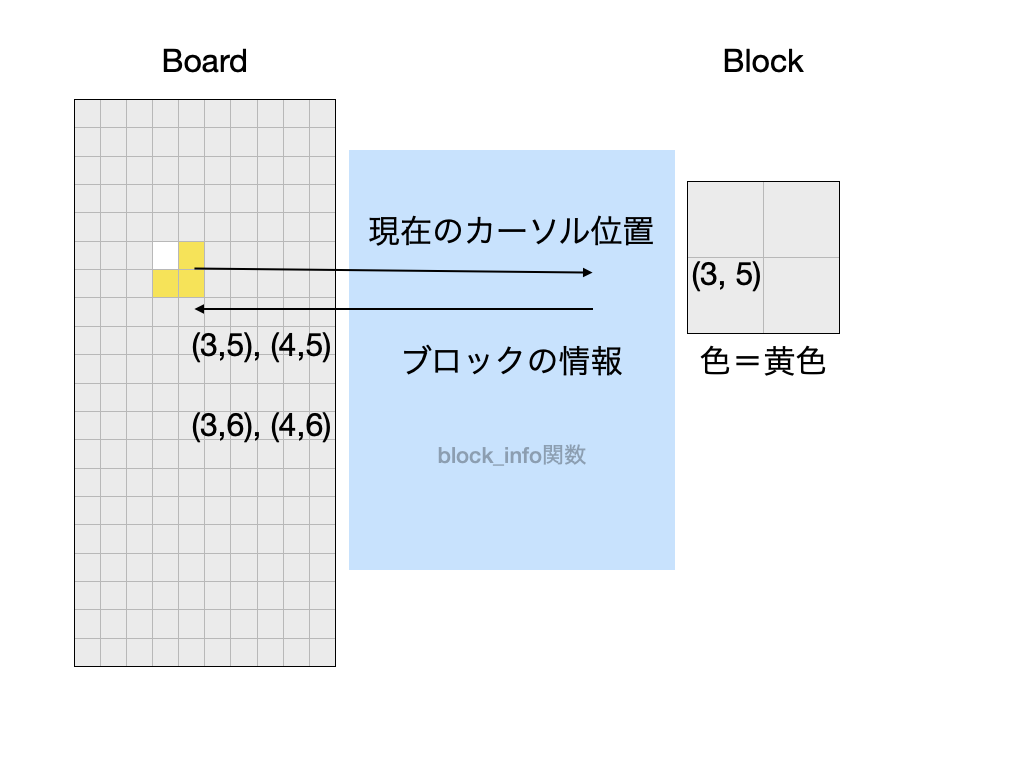
\includegraphics[width=100mm]{images/BoardAndBlock.png}
  \caption{BoardとBlockのやりとり}
\end{figure}

Boardが現在保持中のブロックの変数を持つということなので、Boardクラスに変数を追加します。
最初は何も持っていないので、「動いているブロック」という意味の「moving\_block」にPythonの特別な空を表す「None」を入れておきます。
さらに、ブロックの描画を行う処理をBoardクラスに追加します。画面に書く処理はdraw関数でしたね。
draw関数は現在の盤面を塗る(動かしているブロックは対象外)→カーソルを描く→グリッドを描く、という順番で行われていました。
どこに動かしているブロックを描く処理を入れるか考えてみましょう。
\lstinputlisting[caption={Boardクラスの変更点}, language=Python]{chapter6/ch6_2_1.py}
\texttt{"""..."""}は自分で書いてみましょう。変数の名前を変にしすぎると
先生が助けにくくなります。

\section{ブロックのクラスを定義する}
\subsection{OBlockクラスを定義する}
今回はOブロックを作ります。Oブロックは一番簡単なブロックです。2x2の黄色の正方形です。
最初にこれから作ることにしたのは、回転が必要ないからです。
ブロックにはどのような機能が必要だったか思い出してみます。
\begin{itemize}
  \item ブロックを回転させる関数
  \item 自分の色をもつ変数
  \item ブロックの情報を返す関数
\end{itemize}
\newpage
\lstinputlisting[caption=OBlockクラスの作成, language=Python]{chapter6/ch6_2_2.py}
block\_info関数はカーソルの位置を受け取って、
そこからカーソルの位置、右、下、右下の4つのマスを返します。
Boardはその座標とOBlockの中にあるcolor変数を使って描画します。
rotate関数は今回は作っていませんが、ブロックの種類によっては必要になります。

\section{ブロックを表示させてみる}
\subsection{main関数を変更する}
main関数を変更して、OBlockを動かしてみましょう。
\lstinputlisting[caption={OBlockのテスト}, language=Python]{chapter6/ch6_3_1.py}
うまくいっていれば、Oブロックが動くはずです。
\newpage
\begin{figure}[h]
  \centering
  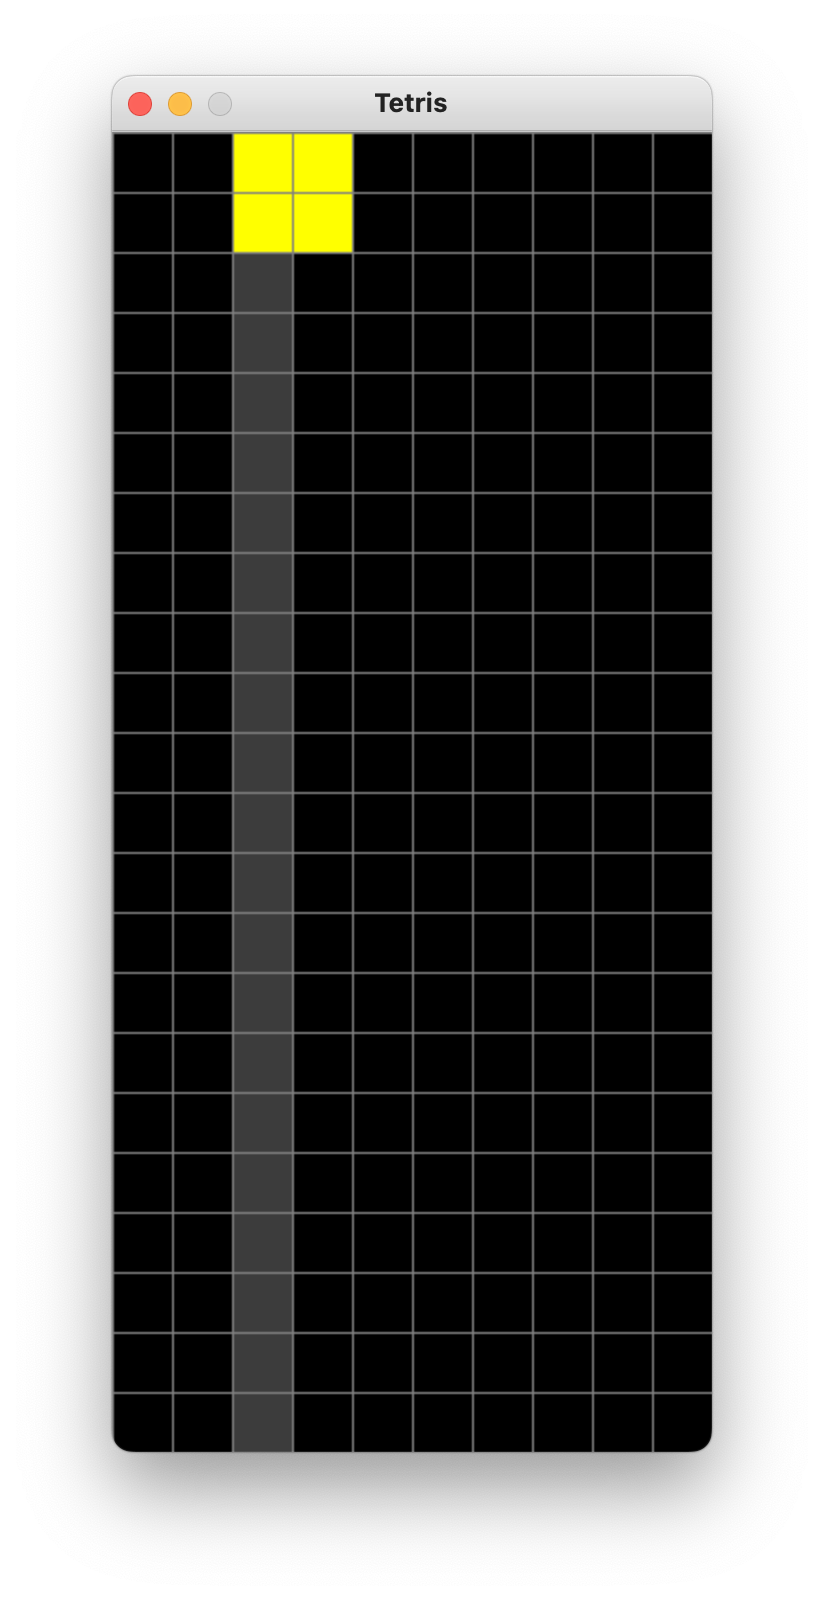
\includegraphics[height=80mm]{images/TetrisCH7.png}
  \caption{テトリスの実行結果}
\end{figure}
\newpage
ここで右端に動いてみましょう。ブロックが半分消えてしまいますね。

\subsection{ブロックの移動範囲を制限する}
この問題を解決するために、ブロックの移動範囲を制限する機能を追加します。
キー入力を受け取ってから動くまでの間に、ブロックが動けるかどうかを判定する処理を入れます。
さて、どこに入れるといいでしょうか?
\subsubsection{設計}
\begin{itemize}
  \item main関数が判定する
  \item Boardが判定する
  \item Cursorが判定する
  \item OBlockが判定する
\end{itemize}
クラスを使う前まではmain関数が判定するのが一般的でした。
しかし、今回はmainには余計な仕事をさせないようにしましょう。
動きを担当するのはCursorの役割です。Cursorにmove\_right関数などを
追加していたはずです。ここを次のように変更することで対処します。
\begin{itemize}
  \item OBlockはCursor, Boardから動けるかどうか計算する
  \item Cursorはその情報をもとに動くかどうか決める
\end{itemize}

\subsection{OBlockクラスを変更する}
OBlockクラスに、動ける範囲を計算する関数を追加します。
\lstinputlisting[caption={OBlockクラスの変更}, language=Python]{chapter6/ch6_3_2.py}
さて、次にカーソルの動きを変更します。
今までは無条件に動いていましたが、一度ブロックを受け取って動けるか
どうかを判定してもらい、動けるなら動くようにします。

\subsection{Cursorクラスを変更する}
\lstinputlisting[caption={Cursorクラスの変更}, language=Python]{chapter6/ch6_3_3.py}
これらの変更が終わると、main.pyにエラーが出ているはずです。
今まではcursor.move\_right()のように書いていましたが、
これからは引数としてboardとblockを渡す必要があるからです。
もちろん、main関数で引数を渡すように変更しても良いのですが、
少し見栄えが悪いので(プログラマとしては見栄えが悪いです)、変更を加えます。
\subsection{Boardクラスを変更する}
今回はカプセル化という方法で、BoardクラスがCursorをカプセルのように閉じ込めて、
Board経由でCursorを操作するようにします。
そこで、Boardクラスにmove\_right関数を追加し、Cursorのmove\_right関数を呼び出すようにします。
\lstinputlisting[caption={Boardクラスの変更}, language=Python]{chapter6/ch6_3_4.py}
\subsection{main関数の変更}
最後に、main関数を変更して、cursorを使うのではなく、boardの移動機能を使うようにします。
\lstinputlisting[caption={main関数の変更}, language=Python]{chapter6/ch6_3_5.py}
これを実行すると、ブロックが右端に行かなくなります。
また、下方向にも消えずに止まるようになります。

\section{まとめ}
今回は、簡単なOBlockを作成しました。Boardクラスにブロックの情報を持たせ、
Boardは適宜OBlockに情報を要求して描画するようにしました。
また、ブロックの移動範囲を制限する機能を追加し、Cursorクラスにその機能を持たせました。
最後に、main関数を変更して、CursorではなくBoardを使ってブロックを動かすようにしました。

\subsubsection{懺悔}
正直にいうとこのテトリスの設計、若干失敗したなあと思っています。
今はBoardがmoving\_blockを持っています。しかし今回の章でいえば、ブロックをCursorの中に持たせるべきでした。
そうであればBoardがCursorをカプセル化する必要もなかった上に設計が簡単になります。
今後ブロックを落とす処理を追加するときを見越してこのような設計にしたのでいいのですが、
果たしてこれが正解だったのか、今後の展開にご期待ください。

\chapter{回転するブロックを作る -- Tブロック}
\section{Tブロック}
今回はTブロックを作ります。Tブロックは、Tの字の形をしています。
Tブロックは、回転が必要なブロックです。回転するためには、ブロックの形を表す変数が必要です。
今回は、ブロックの形を方角と対応させて持つことにしますが、
\textbf{Tブロックの上の横棒が向いている方が方角になる}ようにします。また、カーソルの位置が
Tのくっついているところになるようにします。

\begin{figure}[h]
  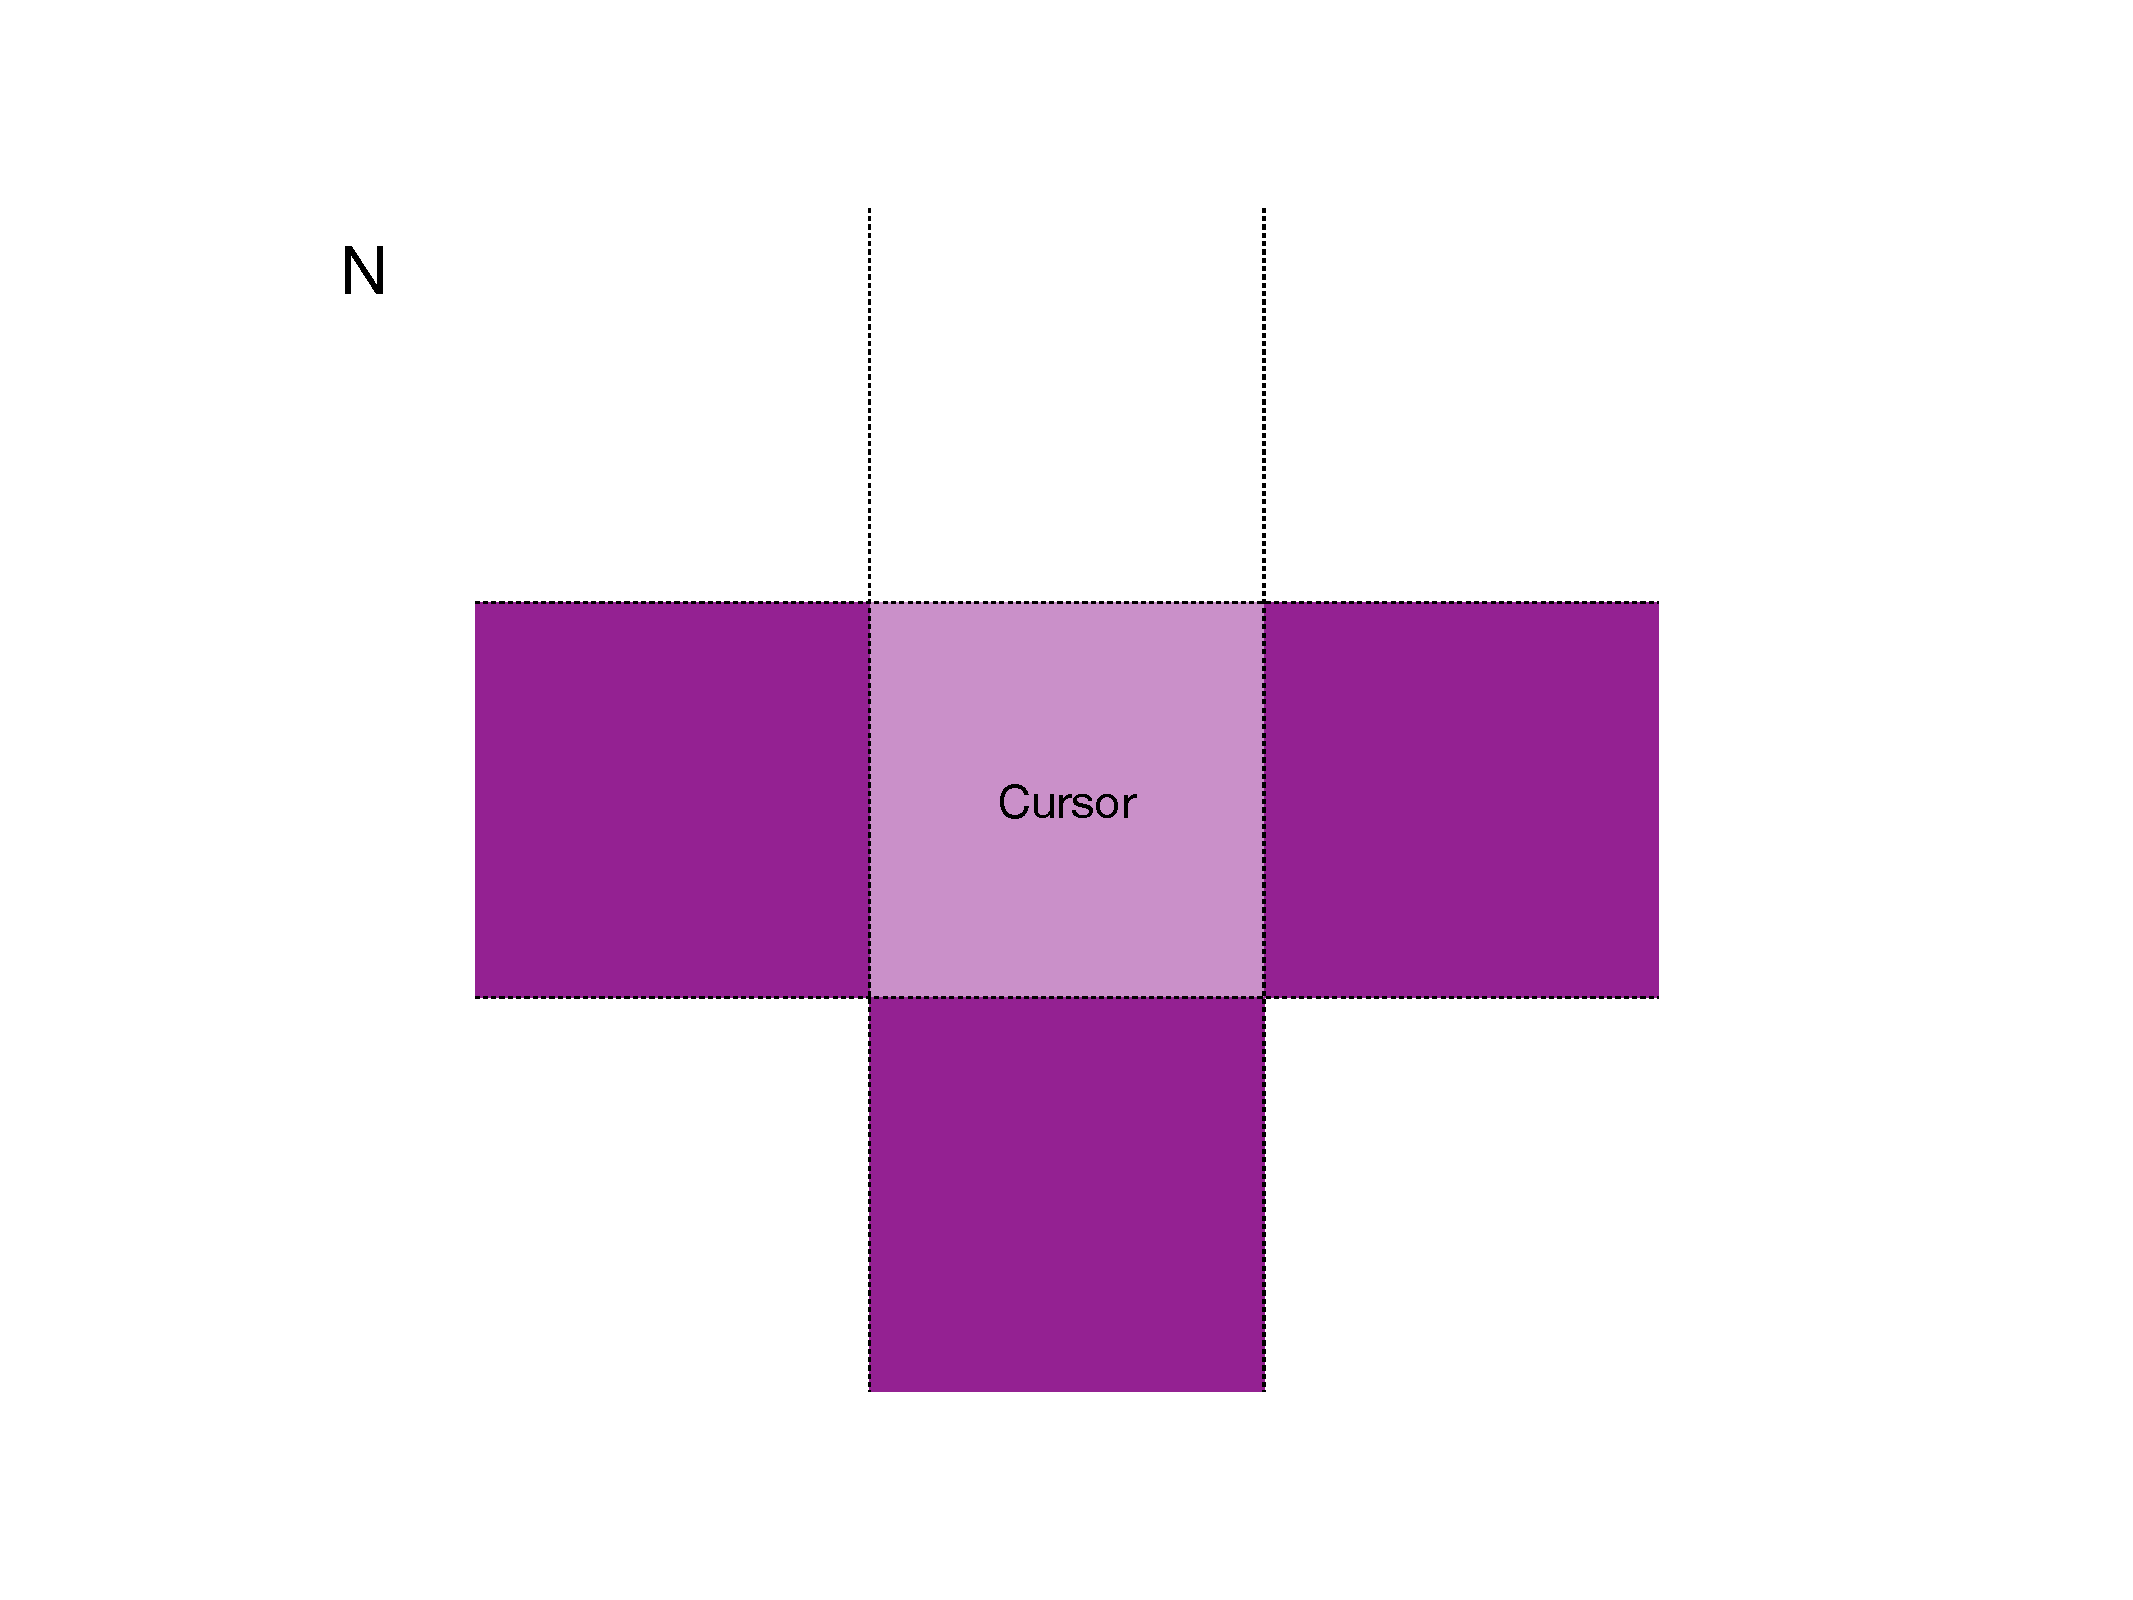
\includegraphics[width=70mm, page=1]{images/Blocks.pdf}
  \includegraphics[width=70mm, page=2]{images/Blocks.pdf}
  \includegraphics[width=70mm, page=3]{images/Blocks.pdf}
  \includegraphics[width=70mm, page=4]{images/Blocks.pdf}
  \caption{Tブロック}
\end{figure}

\newpage
\subsection{Tブロックのプログラム}

\lstinputlisting[caption={Tブロックのプログラム}, language=Python]{chapter7/ch7_1_1.py}

\newpage
\subsubsection{プログラミング豆知識}
回転系、周期系の変数の処理を楽に書きたいときは、それらを0から始まる数字の連番にすることと、
あまりが繰り返すことを利用すると上手く書けます。
\begin{lstlisting}[caption=方角を扱う,language=Python]
N=0
E=1
S=2
W=3
direction = N
direction = (direction + 1) % 4 # directionはE(1)になる
direction = (direction + 1) % 4 # directionはS(2)になる
direction = (direction + 1) % 4 # directionはW(3)になる
direction = (direction + 1) % 4 # directionはN(0)になる、3+1は4だが、4を4で割った余りは0なため
\end{lstlisting}
このように、Nから始まった方角がまたNに戻ってきます。

\subsection{Tブロックの描画}
Tブロックの描画は、Oブロックと同じように行います。
OブロックはBoardにblock\_infoを求められ、その情報をもとに描画していました。
でも、Tブロックもblock\_infoを持っていますから、Oブロックと同じように描画できます。
つまり、\textbf{Boardクラスは変更が必要ありません。オブジェクト指向の利点です。}
違うクラスであっても同じ名前で関数を設計すると、他のクラスから同じように扱えます。
でも中身自体は違うので、それぞれのブロックがそれぞれにあった情報を返すことができるのです。
こういう性質を「ポリモーフィズム/多態性」と言います
\footnote{厳密には違うんですがPythonにポリモーフィズムはあってないようなものなので教えるとしたらこうするしかないんです}。
では、main関数を変更して最初にTブロックを表示してみましょう。
\lstinputlisting[caption={テスト用にTブロックを表示}, language=Python]{chapter7/ch7_2_1.py}
できたら実行しましょう。表示だけで動かすとエラーになります。
\begin{figure}[h]
  \centering
  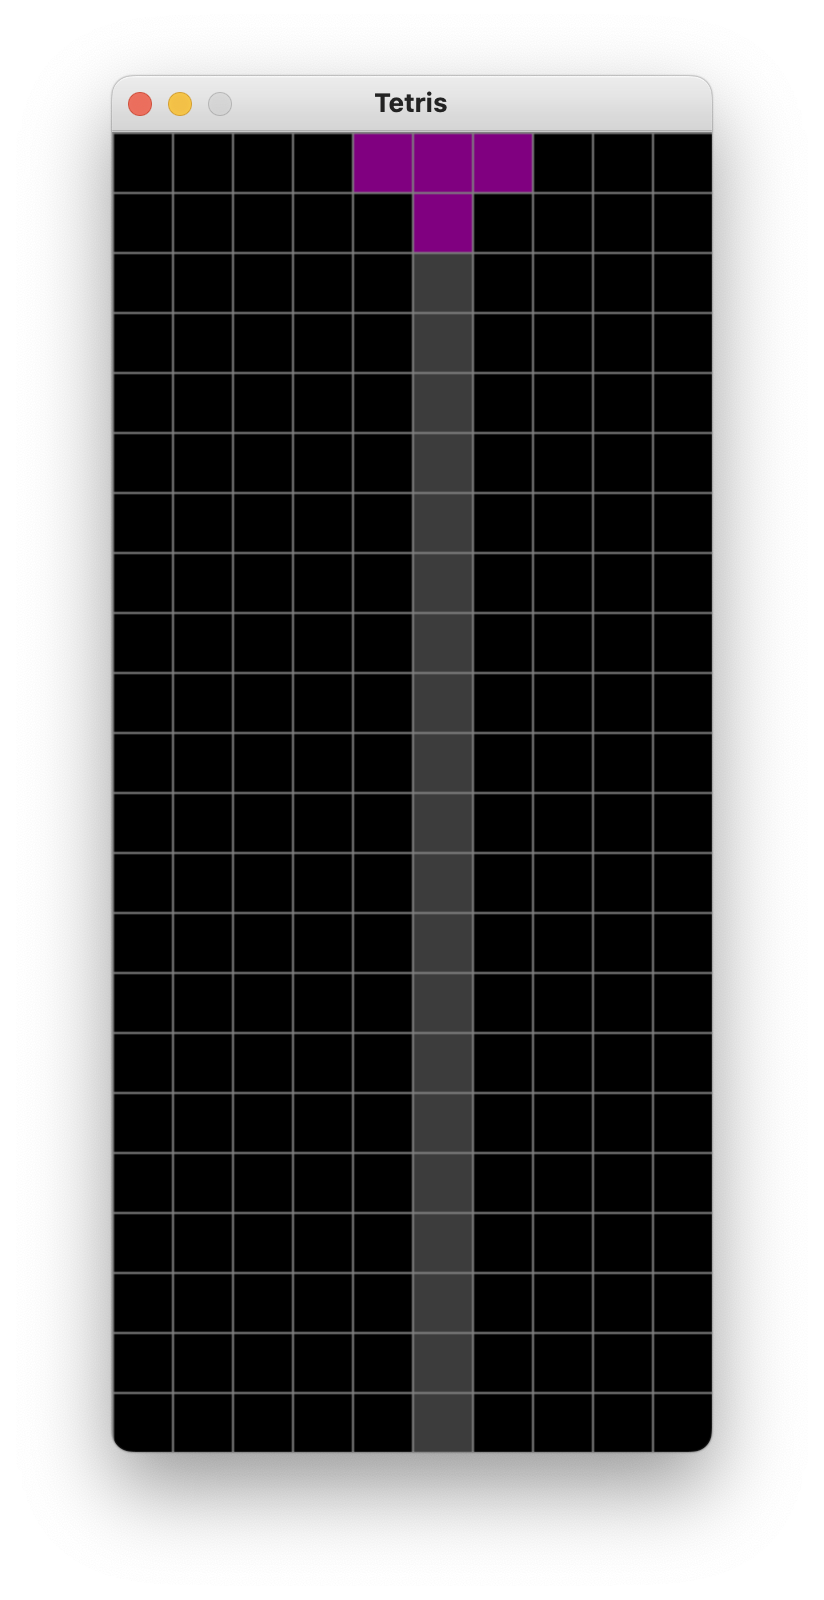
\includegraphics[width=50mm]{images/CH7_2.png}
  \caption{Tブロックの表示}
\end{figure}

\section{Tブロックを動かす}
なぜエラーになったのでしょうか?それは、Tブロックが動けるかどうかを判定する機能がないからです。
Oブロックは動けるかどうかを判定する機能を持っていましたが、Tブロックにはありません。
Boardはそのことを知らずにその関数を呼び出してしまったためエラーになります。
Tブロックにも動けるかどうかを判定する機能を追加しましょう。
\subsection{Tブロックに動けるかどうかを判定する機能を追加する}
TブロックにもOブロックと同じように、動けるかどうかを判定する機能を追加します。
\lstinputlisting[caption={Tブロックに動けるかどうかを判定する機能を追加}, language=Python]{chapter7/ch7_3_1.py}

\subsection{あれ、回転は?}
main関数でキー入力を受け取っていますので、main関数を実行して回転キーを設定しましょう。

\lstinputlisting[caption={main関数で回転する}, language=Python]{chapter7/ch7_4_1.py}
書き終えたら実行してみましょう。ひとまずお疲れ様でした。でも、まだ終わりではありません。
\begin{figure}[h]
  \centering
  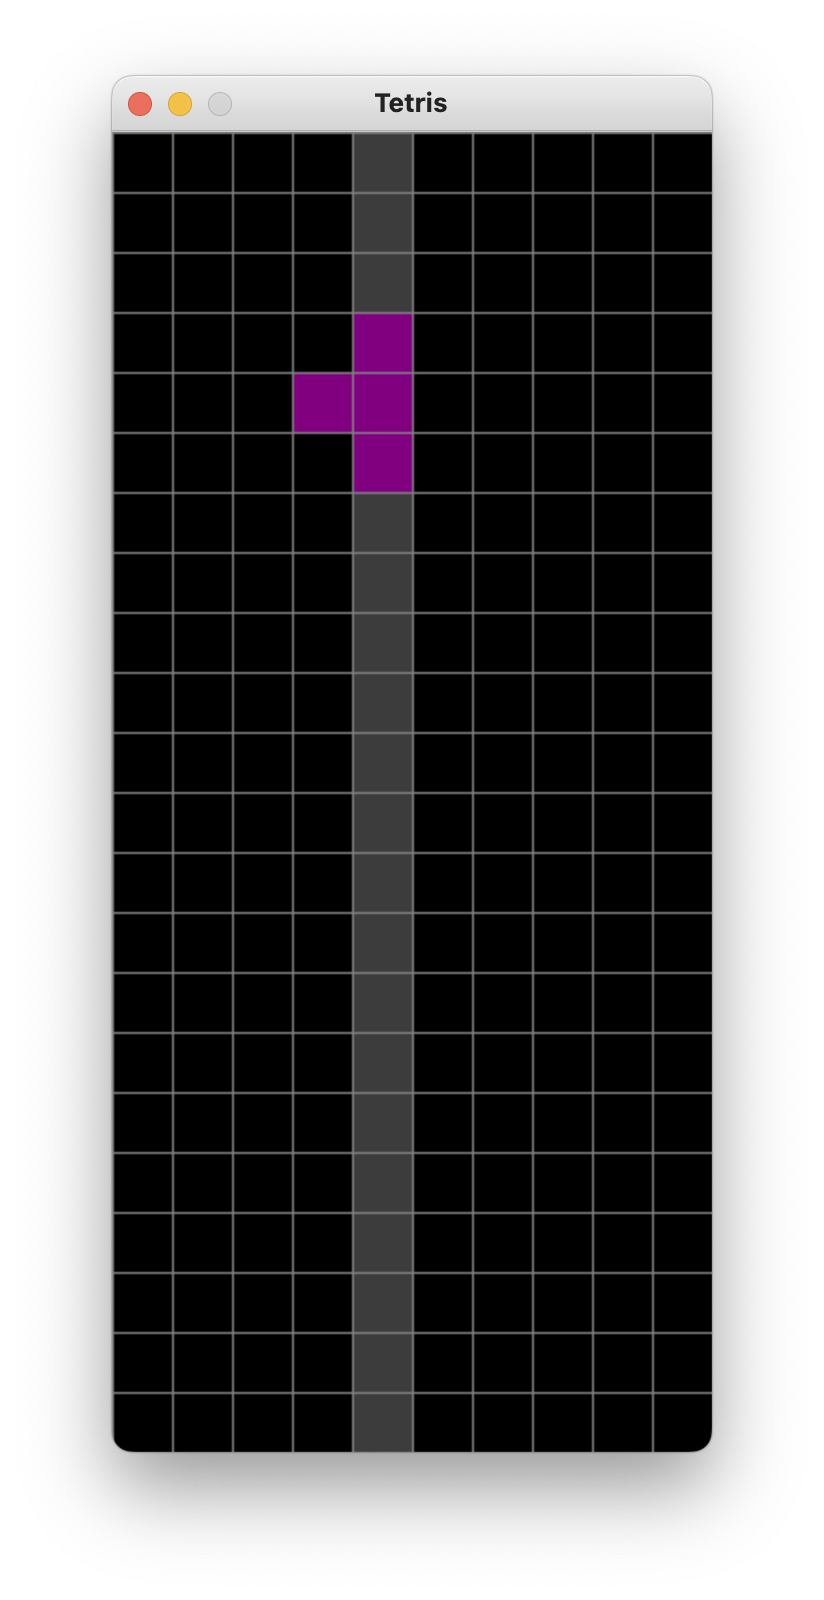
\includegraphics[width=50mm]{images/CH7_4.png}
  \caption{Tブロックの回転}
\end{figure}

回転によりはみ出してしまうことがありますね。これは移動と同じで回転できない状況があるのに、それを検知できずに回転しているからです。

\subsubsection{Q: この教材、いきあたりばったりで作ってないですか?}
多くのメンターさんが共感してくれると思いますが、
基本的にプログラムは一発で動きません。さらに残酷なことに、頑張って書いた時ほど、動かないものです。
ここまできたみなさんには、同じプログラマとして、「せっかく頑張ったのになんでやねん」というこのガッカリ感を
味わってみて欲しいです。

実行する前にこうなることが予期できた人は素晴らしいです。ぜひ、次回以降もこのような予測をしていってください。

\section{回転できるか判定する関数をつくる}
それでは、回転について判定する関数を作ってみましょう。
いくつか方法が考えられますが、今回は、回転した後の座標を計算して、その座標が盤面と衝突しないかどうかを判定する方法を取ります。
\subsection{回転できるか判定する関数をつくる}
以下のように書いてみましょう。戻り値はbool型、すなわちTrueかFalseです。
可能だと分かったらその時点でreturn True、逆に不可能だと分かったらreturn Falseします。
\lstinputlisting[caption={回転できるか判定する関数をつくる}, language=Python]{chapter7/ch7_5_1.py}
ちなみに、もっと賢い方法を思いついた人は、それを書いて試してみましょう。
この教材では直感的な方法をとっています。

次に、\textbf{判定をしてから回転する}部分を作ります。
今回も前回同様に、Boardクラスがブロックの回転する関数を提供します。
\subsection{Boardクラスに回転する関数をつくる}
\lstinputlisting[caption={Boardクラスに回転する関数をつくる}, language=Python]{chapter7/ch7_5_2.py}
これで回転できる時に回転する、機能が完成しました。
最後に、main関数を変更しましょう。
\subsection{main関数を変更する}
\lstinputlisting[caption={main関数を変更する}, language=Python]{chapter7/ch7_5_3.py}
実行すると、Tブロックが正しく回転するようになるはずです。
うまくいかない場合はcan\_rotateが大体間違っていると思うので、先生と相談してください。

\subsubsection{コラム: if \_\_name\_\_ == "\_\_main\_\_"について}
Swimmyの教材には書いていませんが、Pythonには\_\_name\_\_という変数があらかじめ使えます。
もちろん変数なのでprintが可能です。
\begin{lstlisting}[caption=\_\_name\_\_の使い方,language=Python]
print(__name__)
\end{lstlisting}
これを実行すると、\_\_main\_\_と表示されます。これは、このファイルが直接実行されたときに\_\_main\_\_になるということです。
Pythonファイルには、実行する方法が2度あります。
\begin{itemize}
  \item 直接実行する
  \item importして使う
\end{itemize}
importされた時には、\_\_name\_\_はファイル名になります。
import pygameをしたときに
\begin{verbatim}
pygame 2.0.1 (SDL 2.0.14, Python 3.8.3)
Hello from the pygame community. https://www.pygame.org/contribute.html
\end{verbatim}
こんな表示を見たことはありませんか?
おそらく、pygameのファイルにはこんなのが書いてあるはずです
\begin{lstlisting}[caption=pygameのファイルの一部,language=Python]
  print("pygame 2.0.1 (SDL 2.0.14, Python 3.8.3)")
  print("Hello from the pygame community. https://www.pygame.org/contribute.html")
\end{lstlisting}
使い道はかなり限定されていますが、
\begin{itemize}
  \item このファイルが間違ってimportされた時に警告を出したい
  \item importして使って欲しいので直接実行された時はエラーを出したい
  \item バージョンを表示したり、著作権表示をしたい
\end{itemize}
こんな時に使われている傾向があります。
せっかくなので、自分のファイルにも書いてみてください。
\lstinputlisting[language=Python]{chapter7/ch7_5_4.py}
import tetrisのあたりでprintが実行され、自分の名前が出てくるはずです。

\section{まとめ}
今回はTブロックを作りました。TブロックはOブロックと違い、回転が必要なブロックです。
そのため、回転できるかどうかを判定する機能を追加しました。

\chapter{他のブロックを作る}
\section{LBlockクラス}
今までのTブロックを元に、Lブロックを作ります。
\begin{figure}[h]
  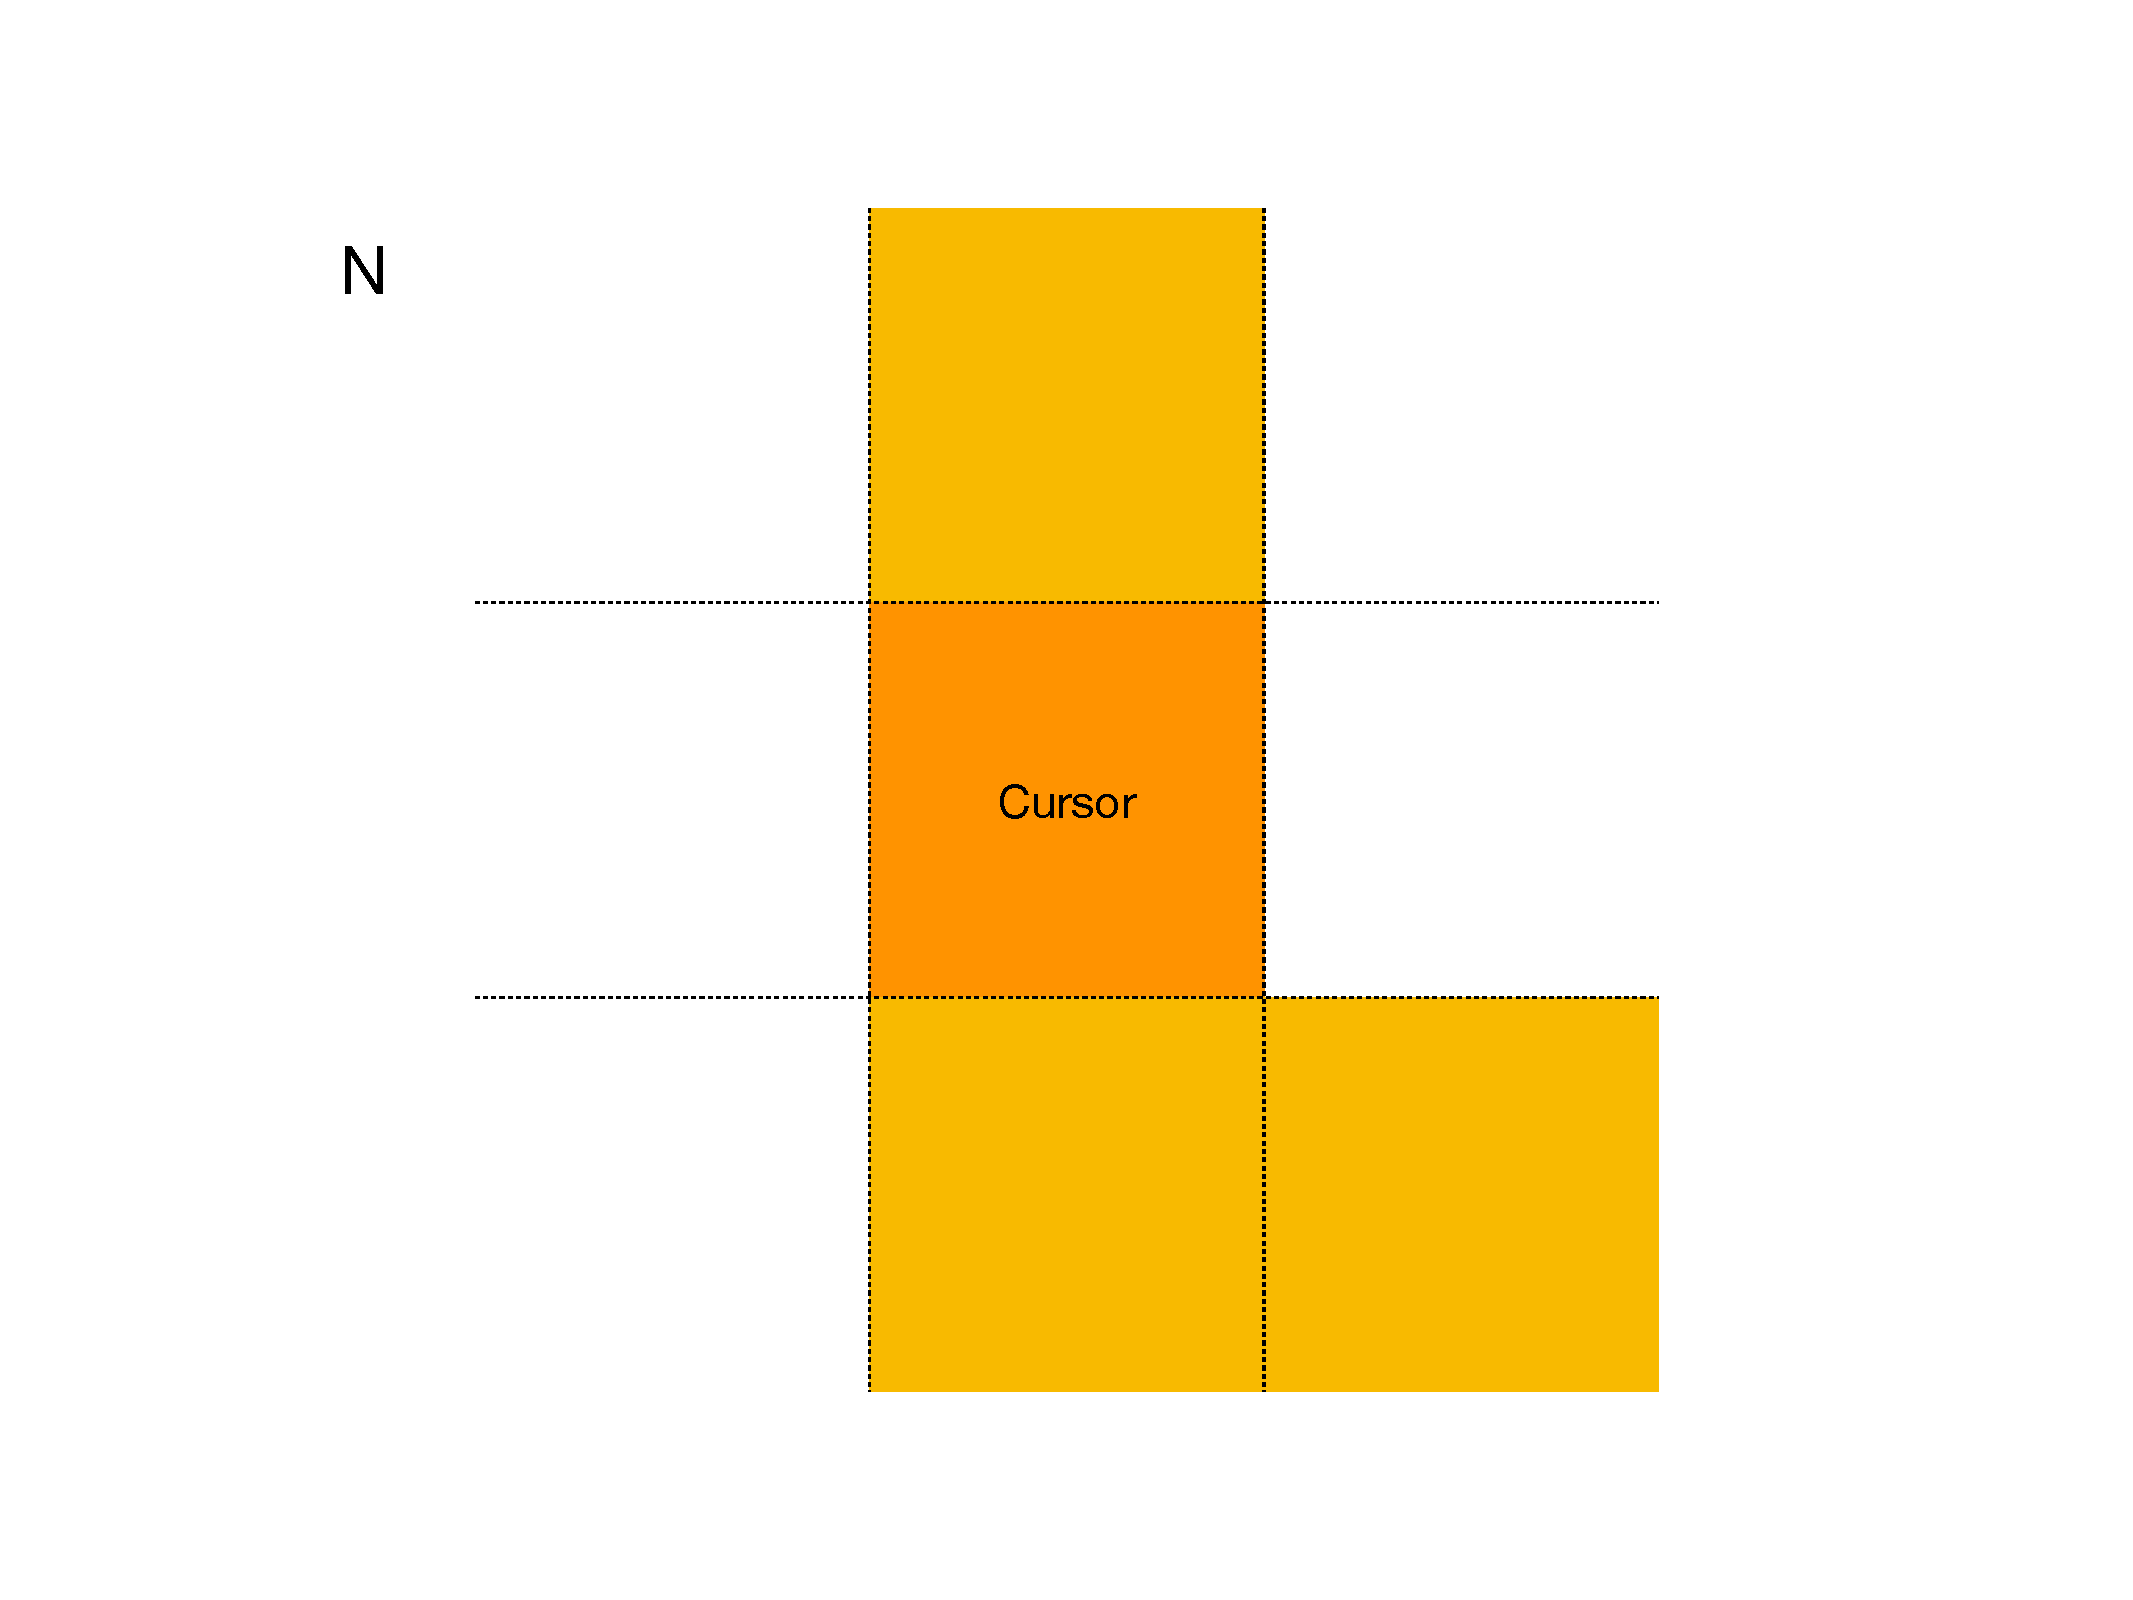
\includegraphics[width=60mm, page=1]{images/LBlock.pdf}
  \includegraphics[width=60mm, page=2]{images/LBlock.pdf}
  \includegraphics[width=60mm, page=3]{images/LBlock.pdf}
  \includegraphics[width=60mm, page=4]{images/LBlock.pdf}
  \caption{Lブロック}
\end{figure}
クラス名はLBlockとしましょう。色はオレンジが多いようです。
以下の関数を作るのを忘れないでください。
\begin{itemize}
  \item block\_info関数 ... カーソルの位置から自分のブロックの様子を座標のリストで返します。
  \item rotate関数 ... 回転します。回転できるかは気にせず、とりあえずselfに入っているrotationという変数を変えるだけにします。
  \item can\_rotate関数 ... 実際に回転したときにはみ出さないか、他のブロックとぶつからないか判定します。引数cursorで現在の位置を、引数board\_infoで盤面の情報を取得します。
  \item can\_go\_up関数 ... 上に移動できるか判定します。引数cursorで現在の位置を、引数board\_infoで盤面の情報を取得します。
  \item can\_go\_down関数 ... 下に移動できるか判定します。引数cursorで現在の位置を、引数board\_infoで盤面の情報を取得します。
  \item can\_go\_right関数 ... 右に移動できるか判定します。引数cursorで現在の位置を、引数board\_infoで盤面の情報を取得します。
  \item can\_go\_left関数 ... 左に移動できるか判定します。引数cursorで現在の位置を、引数board\_infoで盤面の情報を取得します。
\end{itemize}
出来上がったら、main関数で表示してみましょう。
main.pyのmoving\_block = の部分を変更したらできるはずです。

\section{JBlockクラス}
次にJブロックを作ります。
\begin{figure}[h]
  \includegraphics[width=60mm, page=9]{images/Blocks.pdf}
  \includegraphics[width=60mm, page=10]{images/Blocks.pdf}
  \includegraphics[width=60mm, page=11]{images/Blocks.pdf}
  \includegraphics[width=60mm, page=12]{images/Blocks.pdf}
  \caption{Jブロック}
\end{figure}
関数も同じものを作ります。
自分を信じすぎず、一つブロックを作ったらきちんと表示、回転、移動ができるか確認しましょう。

\newpage
\section{SBlockクラス}
次にSブロックを作ります。
\begin{figure}[h]
  \includegraphics[width=60mm, page=13]{images/Blocks.pdf}
  \includegraphics[width=60mm, page=14]{images/Blocks.pdf}
  \includegraphics[width=60mm, page=15]{images/Blocks.pdf}
  \includegraphics[width=60mm, page=16]{images/Blocks.pdf}
  \caption{Sブロック}

\end{figure}
関数も同じものを作ります。

\newpage
\section{ZBlockクラス}
次にZブロックを作ります。
\begin{figure}[h]
  \includegraphics[width=60mm, page=17]{images/Blocks.pdf}
  \includegraphics[width=60mm, page=18]{images/Blocks.pdf}
  \includegraphics[width=60mm, page=19]{images/Blocks.pdf}
  \includegraphics[width=60mm, page=20]{images/Blocks.pdf}
  \caption{Zブロック}
\end{figure}

\newpage
\section{IBlockクラス}
最後にIブロックを作ります。
\begin{figure}[h]
  \includegraphics[width=60mm, page=21]{images/Blocks.pdf}
  \includegraphics[width=60mm, page=22]{images/Blocks.pdf}
  \includegraphics[width=60mm, page=23]{images/Blocks.pdf}
  \includegraphics[width=60mm, page=24]{images/Blocks.pdf}
  \caption{Iブロック}
\end{figure}
うまく動いていることが確認できたでしょうか。
ブロックはこれで全てです。お疲れ様でした。


\chapter{ブロックの落下とランダムなブロックの生成}
\section{ブロックの落下}
今までのプログラムでは、ブロックが動くのはキー入力を受け取ったときだけでした。
しかし、テトリスでは一定時間ごとにブロックが落ちてくるようになっています。
今回は1秒に一度ブロックが落ちるようにしましょう。
\subsection{1秒ごとに落とす}
1秒を測るためには、時間を計測する必要があります。
今回、main関数のwhile文は一秒間に60回実行されています。
つまり、1秒を測るためには60回のループを数えればいいということです。
\lstinputlisting[caption={main関数を変更する}, language=Python]{chapter9/ch9_1_1.py}
これを実行すると、1秒ごとにブロックが落ちていくようになります。

\subsection{ブロックを落とす}
Boardクラスにdrop関数を追加します。
dropとは、落とす、こぼす、という意味があります。
落ちれなくなるところまで落とすという関数です。
\lstinputlisting[caption={Boardクラスにdrop関数を追加する}, language=Python]{chapter9/ch9_1_2.py}
また、main関数を変更して、スペースキーでブロックを落とせるようにします。
\lstinputlisting[caption={main関数を変更する}, language=Python]{chapter9/ch9_1_3.py}
きちんと動いているでしょうか。

\section{ランダムなブロックの生成}
今度はランダムにブロックを生成する機能を追加します。
generate\_block関数を作り、その中でランダムにブロックを生成するようにします\footnote{generate: 生成する}。
その関数は\_\_init\_\_関数の中で呼び出すと、最初のブロックがランダムになります。
\lstinputlisting[caption={ランダムなブロックの生成}, language=Python]{chapter9/ch9_2_1.py}
これで、ランダムなブロックが生成されるようになりました。
mainでブロックを設定する必要がなくなったので、消してしまいましょう。
\lstinputlisting[caption={main関数の変更}, language=Python]{chapter9/ch9_2_2.py}
これで、ランダムなブロックが生成されるようになりました。
しかし、ブロックが一番下まで落ちても、次のブロックに切り替わりません。
次の章でその機能を追加します。

\chapter{次のブロックへ切り替える}
\section{ブロックが一番下まで落ちた時とは}
ブロックがこれ以上下に落ちられないとき、次のブロックに切り替える処理を書きます。
現在、1秒に一回、ブロックが落ちるようになっているので、そこを利用しましょう。
\begin{figure}[h]
  \centering
  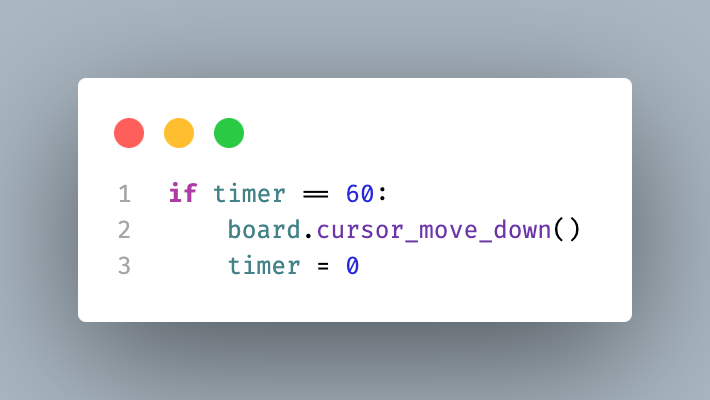
\includegraphics[width=100mm]{images/timer.png}
  \caption{「一秒経った時」を実現しているif文}
\end{figure}

\subsection{Boardクラスに新しい関数updateを追加}
Boardクラスに新しい関数updateを追加します。
mainに「もしブロックが…」のような処理を書いても動きはするのですが、
役割分担の考え方からBoardクラスに書くことにします。
\lstinputlisting[caption={定期的にブロックを落とし、落とせないなら次のブロックを用意するupdate関数}, language=Python]{chapter10/ch10_1_1.py}
次に、main関数を変更します。今まで単純にブロックを落としていた部分をupdate関数に変更します。
\lstinputlisting[caption={main関数を変更する}, language=Python]{chapter10/ch10_1_2.py}
実行すると、ブロックが一番下まで落ちたら次のブロックに切り替わるようになります。

\section{ブロックを積む}
前回のセクションでは、ブロックが切り替わった時に前のブロックが消えてしまう問題がありました。
今回は、ブロックが一番下まで落ちた時に、そのブロックを置く処理を書きます。
\subsection{Boardクラスにfix関数を追加}
Boardクラスにfix関数を追加します\footnote{fix: 固定する、直す}。
ここで、盤面がどのように描かれているかを復習します。
\subsubsection{スクリーンへの書き込みを行なっている場所}
実際にウィンドウへの書き込みを行なっているのは、draw関数です。
その中でも、\textbf{2~5行目が盤面の描画}、7~9行目がカーソルを灰色にする処理、
14~36行目が現在持っているブロックの描画、42~45行目が枠線の描画になっています。
\begin{figure}
  [h]
  \centering
  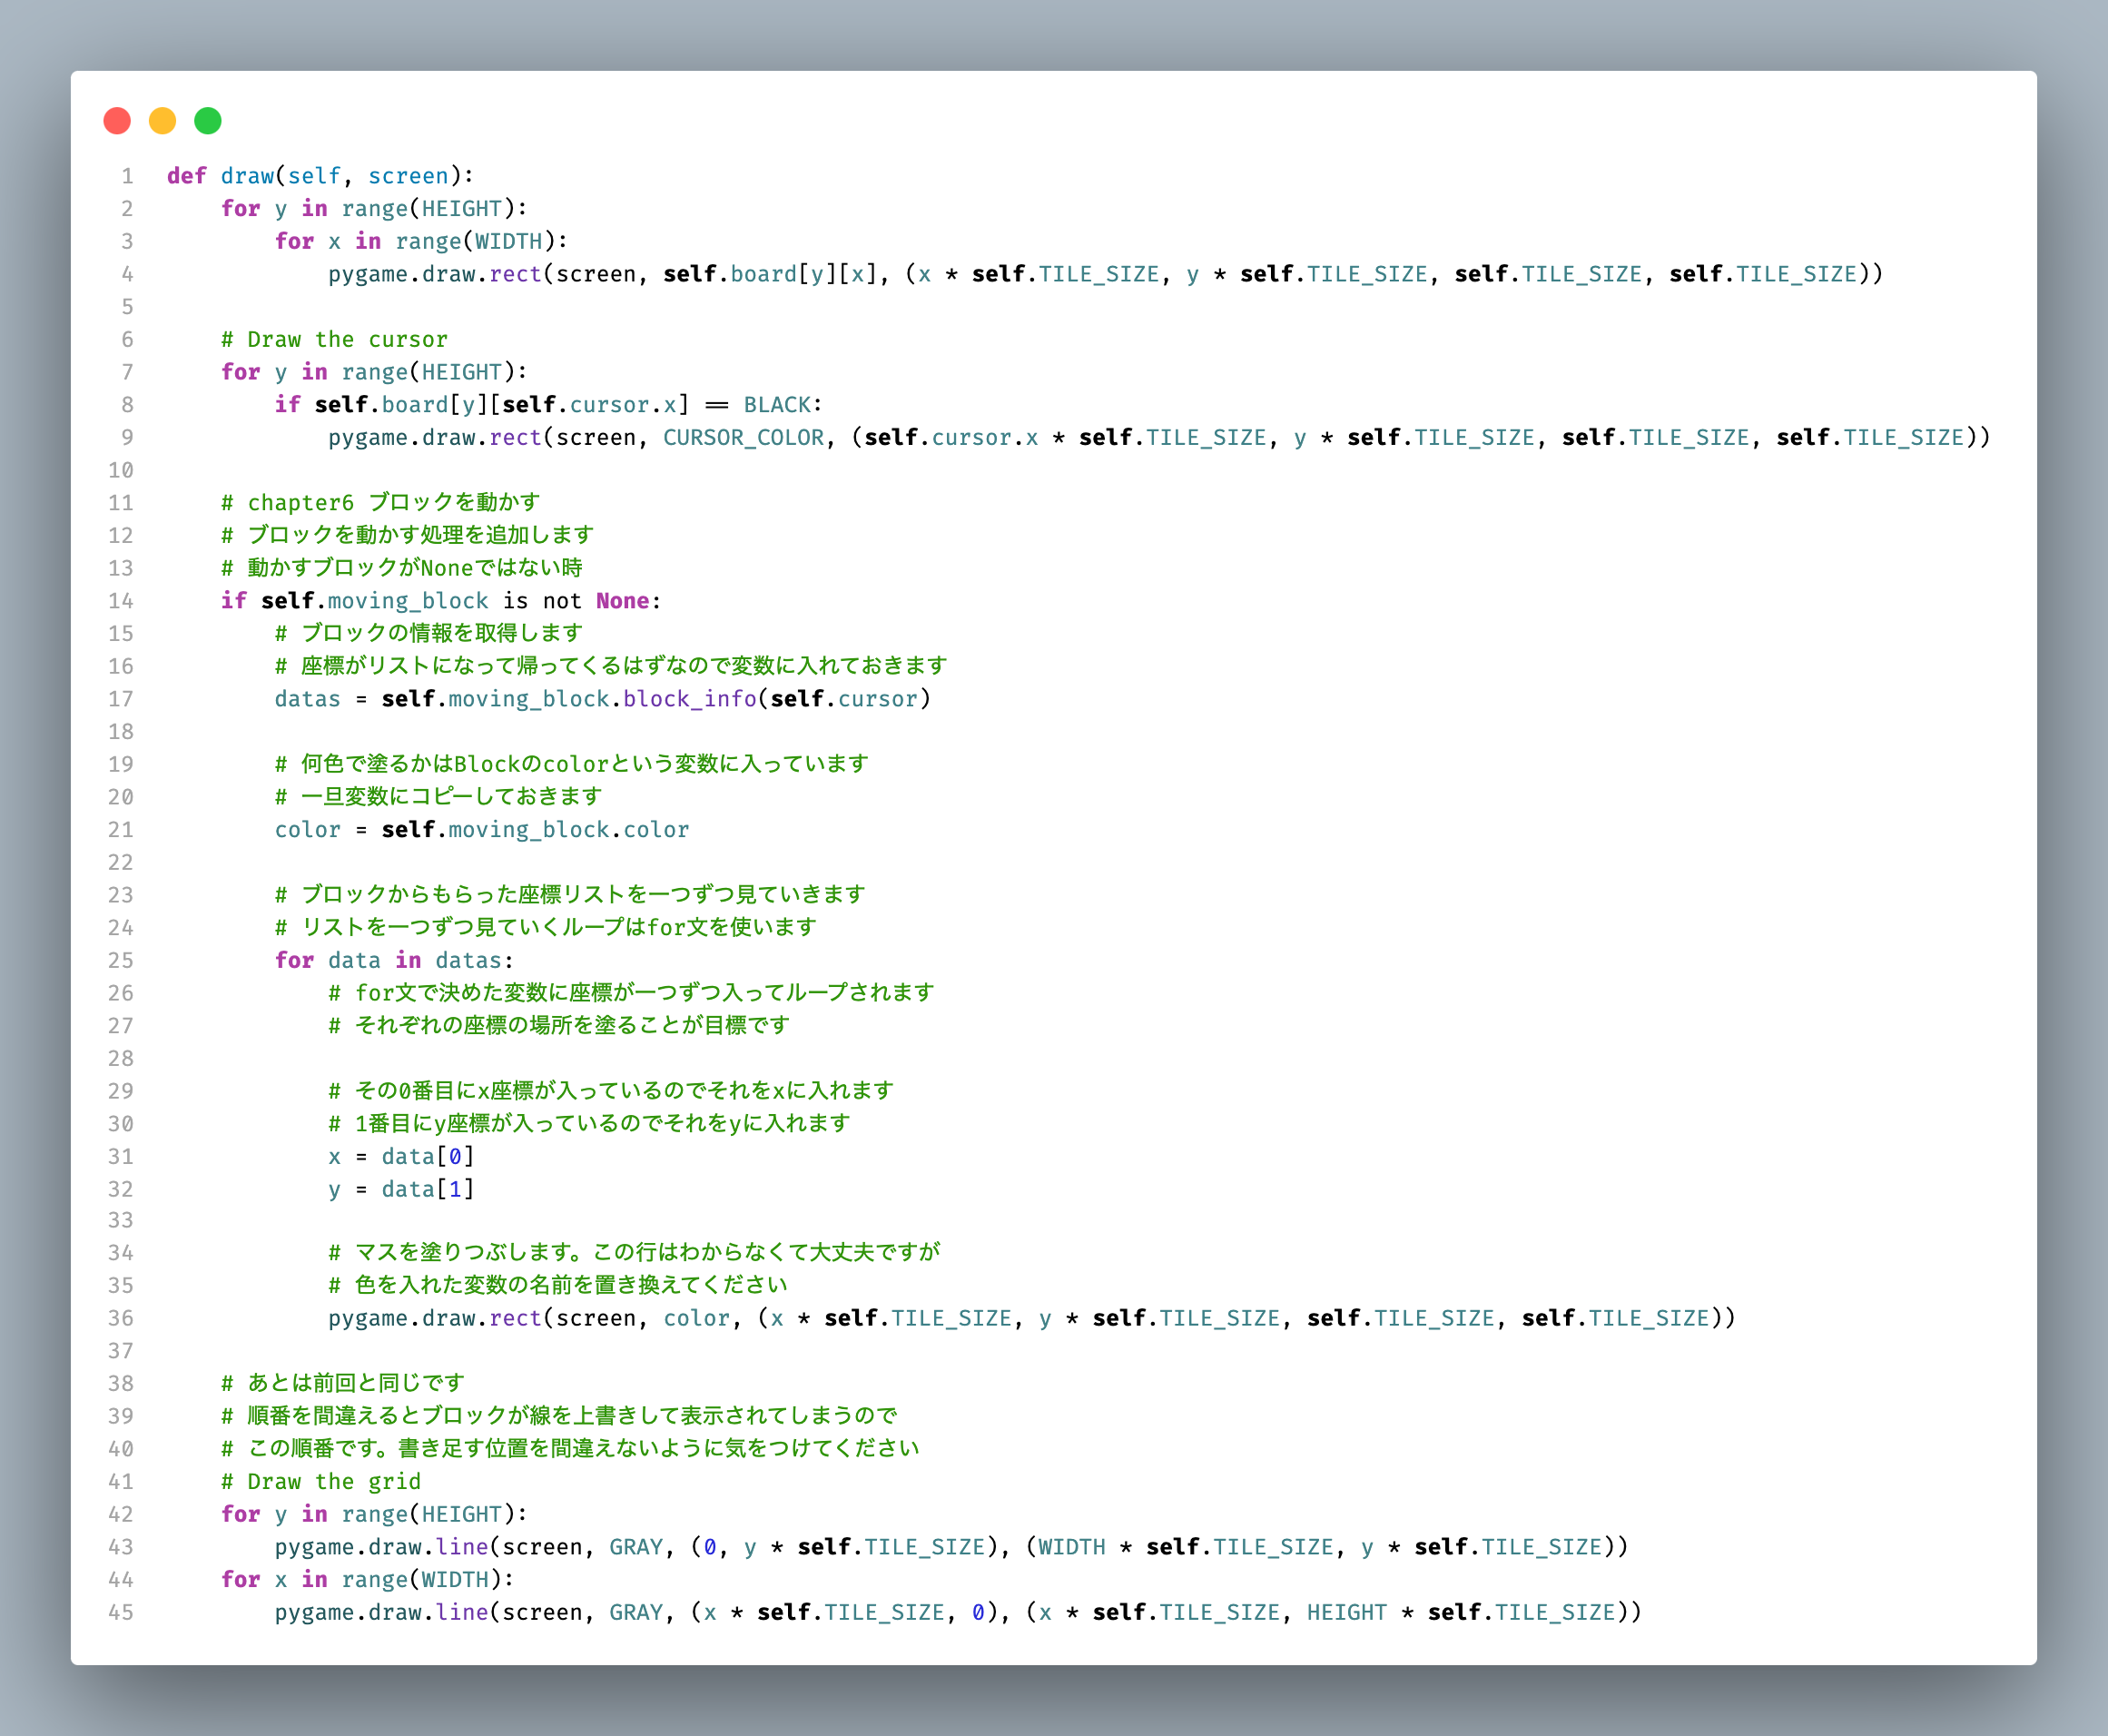
\includegraphics[width=100mm]{images/DrawFunction.png}
  \caption{draw関数の中身}
\end{figure}
ここから、self.boardの中身を変更すれば、draw関数が自動的に画面に反映してくれそうです。
\begin{figure}
  [h]
  \centering
  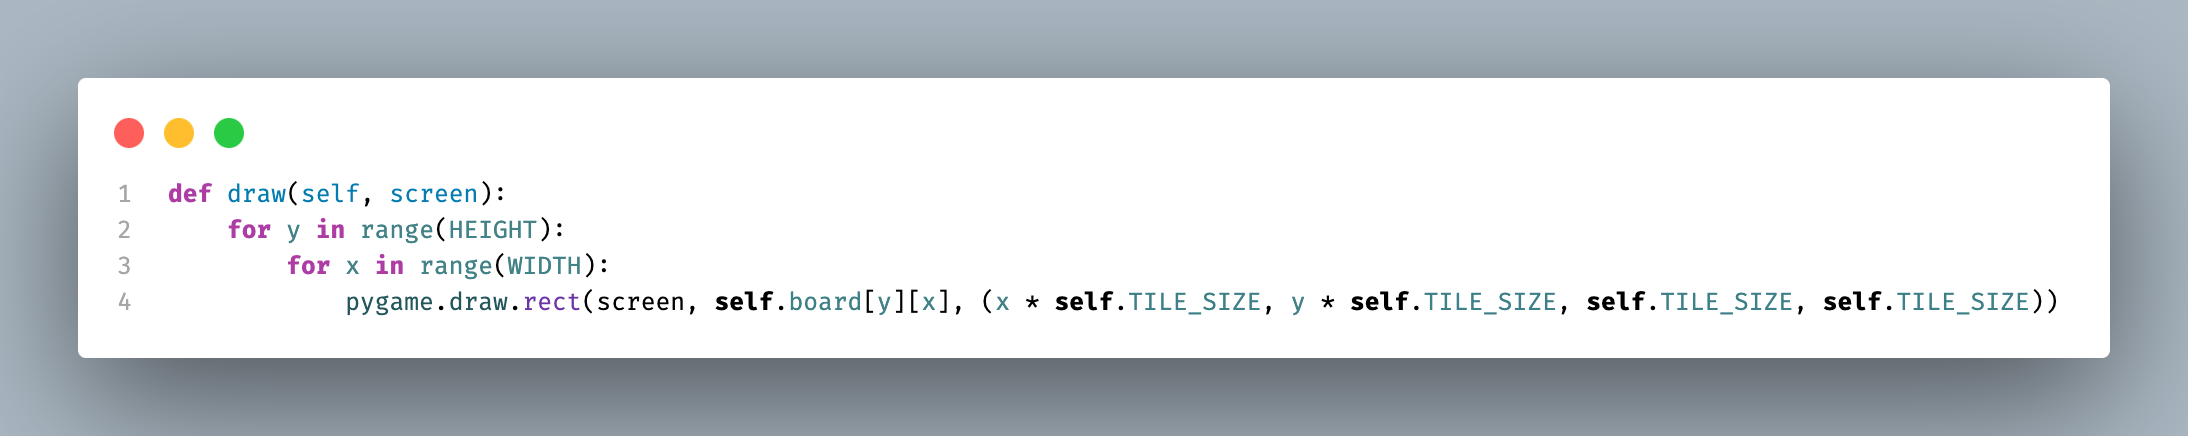
\includegraphics[width=\textwidth]{images/DrawBoard.png}
  \caption{self.boardを変更すれば画面にも反映されそう}
\end{figure}

\subsection{fix関数を実装}
fix関数を実装します。
\lstinputlisting[caption={fix関数}, language=Python]{chapter10/ch10_2_1.py}
次に、update関数を変更します。
\lstinputlisting[caption={update関数を変更}, language=Python]{chapter10/ch10_2_2.py}
実行すると、ブロックが一番下まで落ちたら、そのブロックが盤面に固定されるようになります。

%\chapter{行を消す}
\section{盤面を確認して行を消す関数erase\_lines}
盤面を確認して、揃った行を消す関数erase\_linesを作ります。
盤面は、self.boardに2次元配列として保存されています。
配列の配列は下のようなイメージです。

\end{document}